\documentclass[conference]{IEEEtran}
\usepackage[utf8]{inputenc}
\usepackage{graphicx}
\usepackage{booktabs}
\usepackage{float}
\usepackage{hyperref}
\usepackage{amsmath}
\usepackage{cite}

\title{Perbandingan Kinerja CNN from Scratch dan Transfer Learning untuk Klasifikasi Gambar}

\author{
  \IEEEauthorblockN{~}
  \IEEEauthorblockA{M. Faridh Maulana \textit{452024611065}\\
    Program Studi Teknik Informatika, Universitas Darussalam Gontor\\
    Email: mfaridhmaulana47@student.cs.unida.gontor.ac.id\\
  }
}

\begin{document}

\maketitle

\begin{abstract}
	Laporan ini menyajikan perbandingan antara dua pendekatan klasifikasi gambar: CNN from scratch dan transfer learning menggunakan ResNet50. Eksperimen pertama menggunakan dataset CIFAR-10 (10 kelas, 50.000 gambar) dengan arsitektur CNN sederhana 2 layer konvolusi. Eksperimen kedua menggunakan dataset Cats vs Dogs (2 kelas, 1.000 gambar) dengan transfer learning ResNet50 yang telah dipretrain pada ImageNet. Hasil menunjukkan CNN from scratch mencapai akurasi 76,76\% pada CIFAR-10, sedangkan transfer learning mencapai 99,50\% pada dataset Cats vs Dogs. Analisis mendalam dilakukan untuk menentukan kapan masing-masing pendekatan paling tepat digunakan berdasarkan ukuran dataset, kemiripan domain, dan ketersediaan komputasi.
\end{abstract}

\section{Pendahuluan}
Klasifikasi gambar merupakan salah satu tugas fundamental dalam computer vision. Convolutional Neural Network (CNN) telah menjadi metode standar untuk tugas ini. Terdapat dua pendekatan utama dalam membangun model CNN: membangun arsitektur dari awal (CNN from scratch) dan memanfaatkan model yang telah dilatih pada dataset besar (transfer learning).

Setiap pendekatan memiliki kelebihan dan kekurangan. CNN from scratch memberikan fleksibilitas penuh dalam desain arsitektur tetapi membutuhkan dataset besar dan waktu training yang lama. Transfer learning memanfaatkan representasi visual yang telah dipelajari dari dataset besar seperti ImageNet, sehingga lebih efisien untuk dataset kecil.

Laporan ini bertujuan untuk membandingkan kedua pendekatan tersebut melalui dua eksperimen:
\begin{enumerate}
	\item CNN from scratch pada dataset CIFAR-10
	\item Transfer learning dengan ResNet50 pada dataset Cats vs Dogs
\end{enumerate}

\section{Deskripsi Dataset}
\subsection{Dataset CIFAR-10}
CIFAR-10 adalah dataset klasifikasi gambar yang terdiri dari 60.000 gambar berwarna berukuran $32 \times 32$ piksel yang terbagi dalam 10 kelas: pesawat, mobil, burung, kucing, rusa, anjing, katak, kuda, kapal, dan truk. Dataset ini terbagi menjadi 50.000 gambar training dan 10.000 gambar testing. Dari 50.000 gambar training, 45.000 digunakan untuk training dan 5.000 untuk validasi. Dataset ini bersumber dari Canadian Institute for Advanced Research (CIFAR).

\subsection{Dataset Cats vs Dogs}
Dataset Cats vs Dogs merupakan subset dari dataset Kaggle/Microsoft yang dipublikasikan di Zenodo oleh Tue Boesen (2024) dengan lisensi CC-BY-4.0~\cite{zenodo_catsdogs}. Dataset terdiri dari 1.000 gambar training (500 kucing, 500 anjing), 200 gambar validasi (100 kucing, 100 anjing), dan 100 gambar testing (tanpa label). Untuk kebutuhan eksperimen, folder validasi digunakan sebagai testing set, dan data training dibagi menjadi 800 training dan 200 validasi.

\section{Preprocessing Data}
\subsection{CNN from Scratch (CIFAR-10)}
Preprocessing untuk CIFAR-10 meliputi:
\begin{itemize}
	\item \textbf{Rescaling:} Normalisasi piksel ke rentang $[0,1]$ menggunakan \texttt{ToTensor()}.
	\item \textbf{Normalisasi:} Standarisasi dengan mean 0,5 dan std 0,5 untuk setiap kanal RGB.
	\item \textbf{Augmentasi training:} \texttt{RandomHorizontalFlip()} untuk flipping horizontal acak dan \texttt{RandomCrop(32, padding=4)} untuk cropping acak dengan padding 4 piksel.
\end{itemize}

\subsection{Transfer Learning (Cats vs Dogs)}
Preprocessing untuk transfer learning disesuaikan dengan kebutuhan ResNet50:
\begin{itemize}
	\item \textbf{Resize:} Gambar di-resize ke 256 piksel.
	\item \textbf{Crop:} \texttt{RandomResizedCrop(224)} untuk training dan \texttt{CenterCrop(224)} untuk testing.
	\item \textbf{Normalisasi:} Menggunakan mean dan std dataset ImageNet $(0,485; 0,456; 0,406)$ dan $(0,229; 0,224; 0,225)$.
	\item \textbf{Augmentasi:} \texttt{RandomHorizontalFlip()} untuk variasi data training.
\end{itemize}

Dataset Cats vs Dogs disusun ulang dari struktur flat file (\texttt{cat.*.jpg}, \texttt{dog.*.jpg}) menjadi struktur subdirektori kelas (\texttt{train/cat/}, \texttt{train/dog/}) agar kompatibel dengan \texttt{ImageFolder} PyTorch.

\section{Implementasi CNN from Scratch}
\subsection{Arsitektur}
Arsitektur CNN dibangun dengan dua blok konvolusi, masing-masing terdiri dari \texttt{Conv2d}, \texttt{BatchNorm2d}, \texttt{ReLU}, dan \texttt{MaxPool2d}. Setelah flattening, terdapat dua fully connected layer:

\begin{verbatim}
Conv2d(3->16, 3x3, pad=1)
    -> BatchNorm2d
    -> ReLU
    -> MaxPool2d(2)

Conv2d(16->64, 3x3, pad=1)
    -> BatchNorm2d
    -> ReLU
    -> MaxPool2d(2)

Dropout(0.25) -> Flatten
    -> Linear(4096->128)
    -> ReLU
    -> Linear(128->10)
\end{verbatim}

Total parameter: ~535.594.

\subsection{Alasan Desain}
\begin{itemize}
	\item \textbf{Dua layer konvolusi:} CIFAR-10 berukuran $32 \times 32$, resolusi kecil. Dua layer konvolusi sudah cukup untuk mengekstrak pola visual dasar tanpa over-parameterisasi.
	\item \textbf{BatchNorm2d:} Menstabilkan distribusi aktivasi dan mempercepat konvergensi.
	\item \textbf{Filter 16 $\rightarrow$ 64:} Jumlah filter bertambah progresif -- layer awal mendeteksi fitur sederhana, layer lanjutan menangkap kombinasi fitur lebih kompleks.
	\item \textbf{Dropout(0.25):} Regularisasi ringan untuk mencegah ko-adaptasi neuron.
\end{itemize}

\subsection{Hyperparameter Training}
\begin{itemize}
	\item Optimizer: Adam (learning rate = 0,001)
	\item Loss function: CrossEntropyLoss
	\item Batch size: 64
	\item Epoch: 30
	\item Learning rate scheduler: ReduceLROnPlateau (patience = 3, factor = 0,5)
\end{itemize}

\section{Implementasi Transfer Learning}
\subsection{Pemilihan Model: ResNet50}
ResNet50 dipilih karena:
\begin{enumerate}
	\item \textbf{Residual connections:} Skip connections mengatasi vanishing gradient, memungkinkan 50 layer tetap trainable.
	\item \textbf{Performa pada dataset kecil:} Terbukti efektif untuk transfer learning pada dataset berukuran kecil hingga sedang.
	\item \textbf{Efisien secara komputasi:} 25,6 juta parameter, lebih ringan dari VGG16/19 (138 juta).
	\item \textbf{Tersedia di torchvision:} Bobot pretrained ImageNet tersedia langsung.
\end{enumerate}

\subsection{Feature Extraction}
Pada tahap feature extraction, seluruh layer konvolusi ResNet50 dibekukan (\texttt{requires\_grad = False}) dan hanya classifier head yang diganti dan dilatih:

\begin{verbatim}
ResNet50 (frozen)
    -> Linear(2048->256) -> ReLU
    -> Dropout(0.3) -> Linear(256->2)
\end{verbatim}

Dari total 24.033.090 parameter, hanya 525.058 (2,2\%) yang dilatih. Training dilakukan selama 10 epoch dengan Adam (lr = 0,001).

\subsection{Fine-tuning}
Setelah feature extraction, seluruh layer dibuka (\texttt{requires\_grad = True}) untuk fine-tuning dengan learning rate rendah (lr = 1e-5) agar bobot pretrained beradaptasi tanpa merusak representasi yang sudah dipelajari. Training dilakukan selama 15 epoch dengan scheduler ReduceLROnPlateau.

\section{Hasil Eksperimen}
\subsection{CNN from Scratch}
\begin{figure}[H]
	\centering
	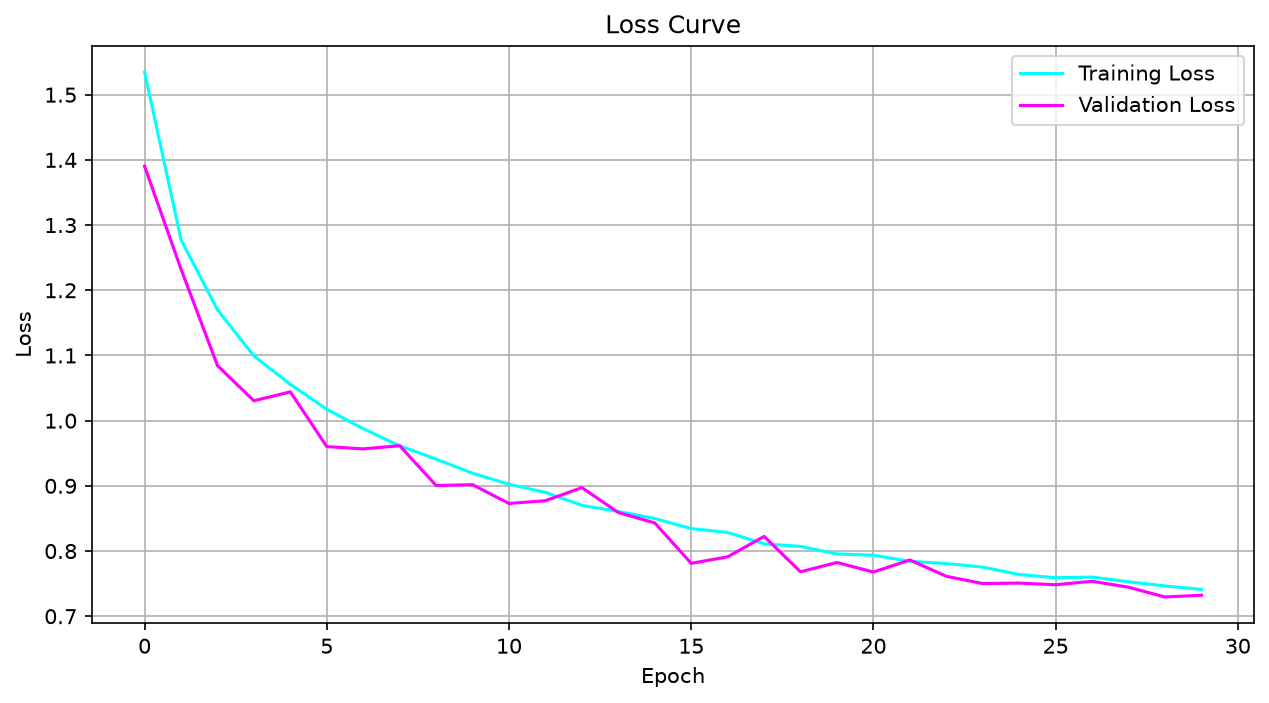
\includegraphics[width=\columnwidth]{figures/loss_curve_cnn_scratch.png}
	\caption{Loss curve CNN from Scratch selama 30 epoch.}
	\label{fig:cnn_loss}
\end{figure}

\begin{figure}[H]
	\centering
	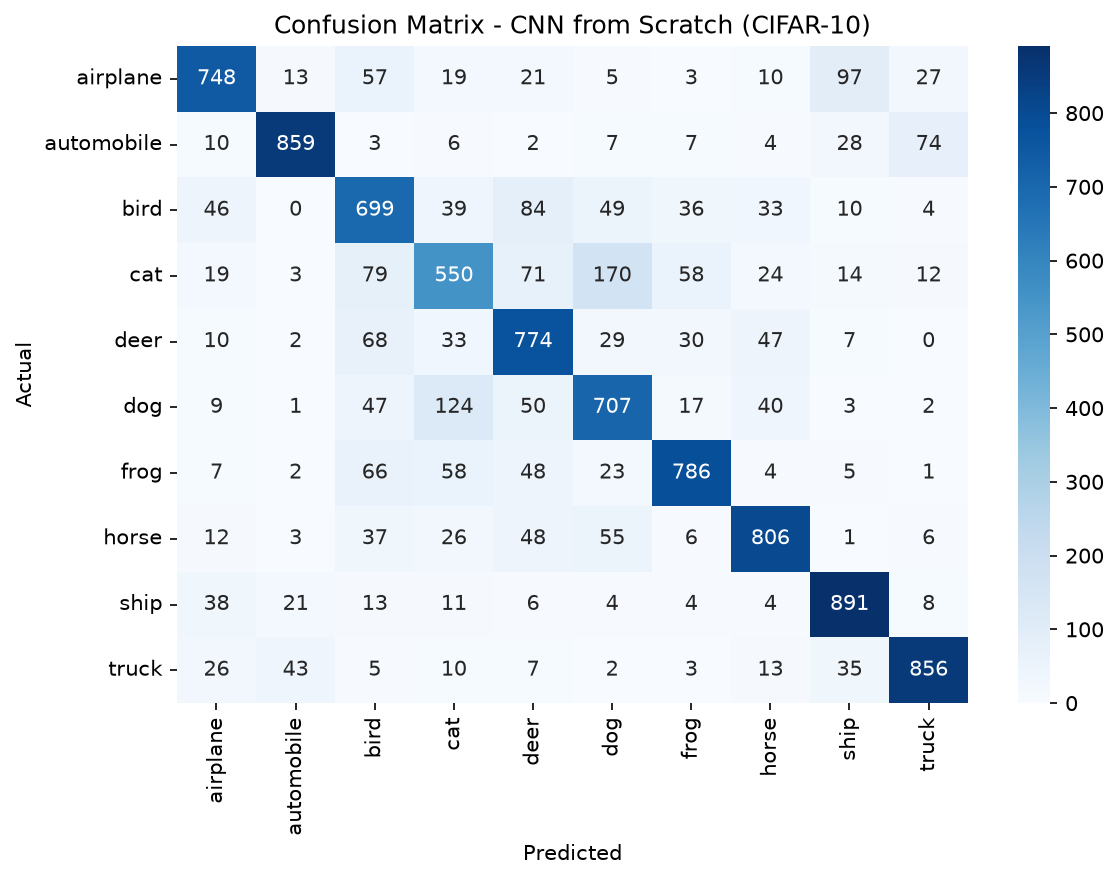
\includegraphics[width=\columnwidth]{figures/confusion_matrix_cnn.png}
	\caption{Confusion matrix CNN from Scratch pada CIFAR-10.}
	\label{fig:cnn_cm}
\end{figure}

\begin{figure}[H]
	\centering
	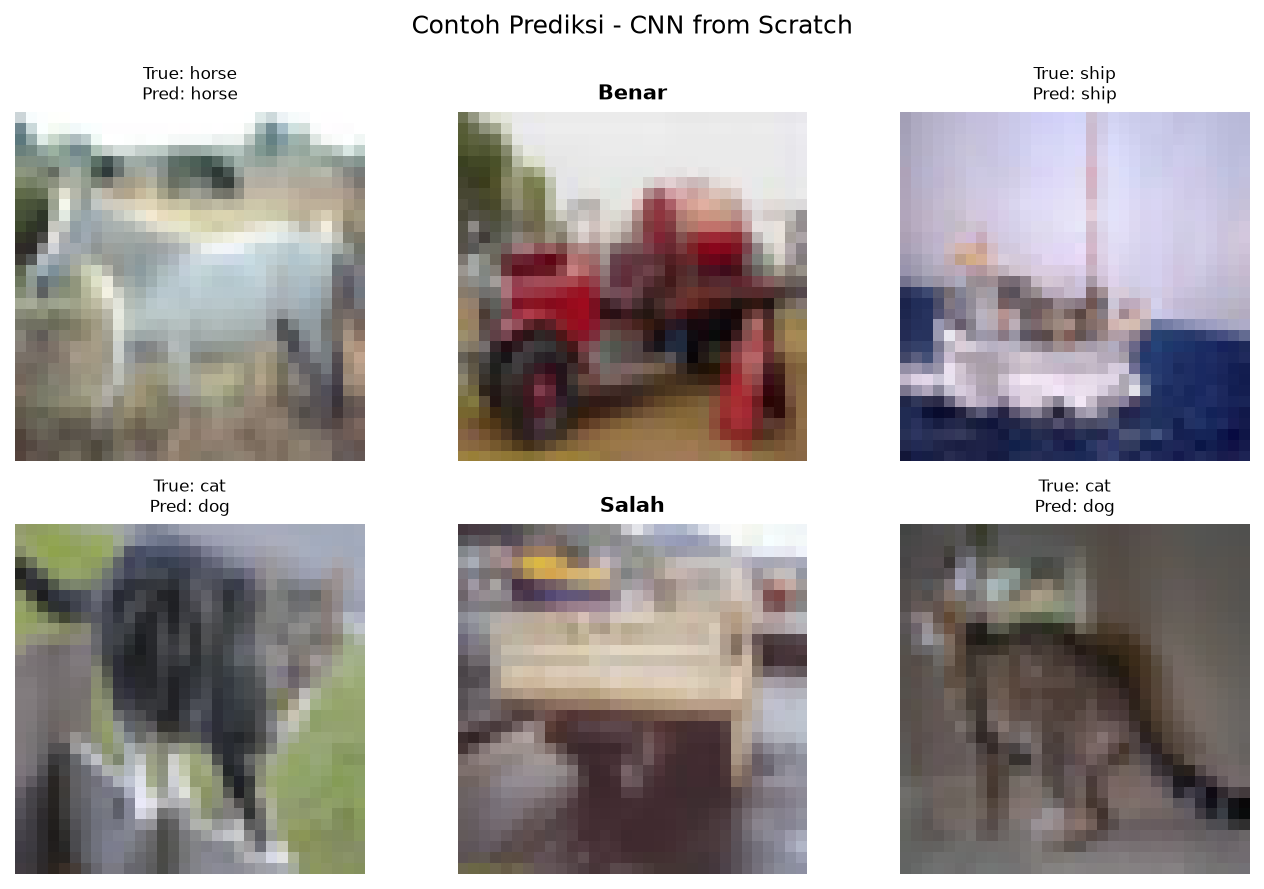
\includegraphics[width=\columnwidth]{figures/predictions_cnn.png}
	\caption{Contoh prediksi benar dan salah CNN from Scratch.}
	\label{fig:cnn_pred}
\end{figure}

CNN from Scratch mencapai akurasi testing sebesar 76,76\% pada dataset CIFAR-10 setelah 30 epoch. Loss training menurun dari 1,53 menjadi 0,74, sementara loss validasi menurun dari 1,39 menjadi 0,73. Tidak terlihat tanda overfitting yang signifikan -- loss validasi mengikuti pola yang sama dengan loss training.

\subsection{Transfer Learning}
\begin{figure}[H]
	\centering
	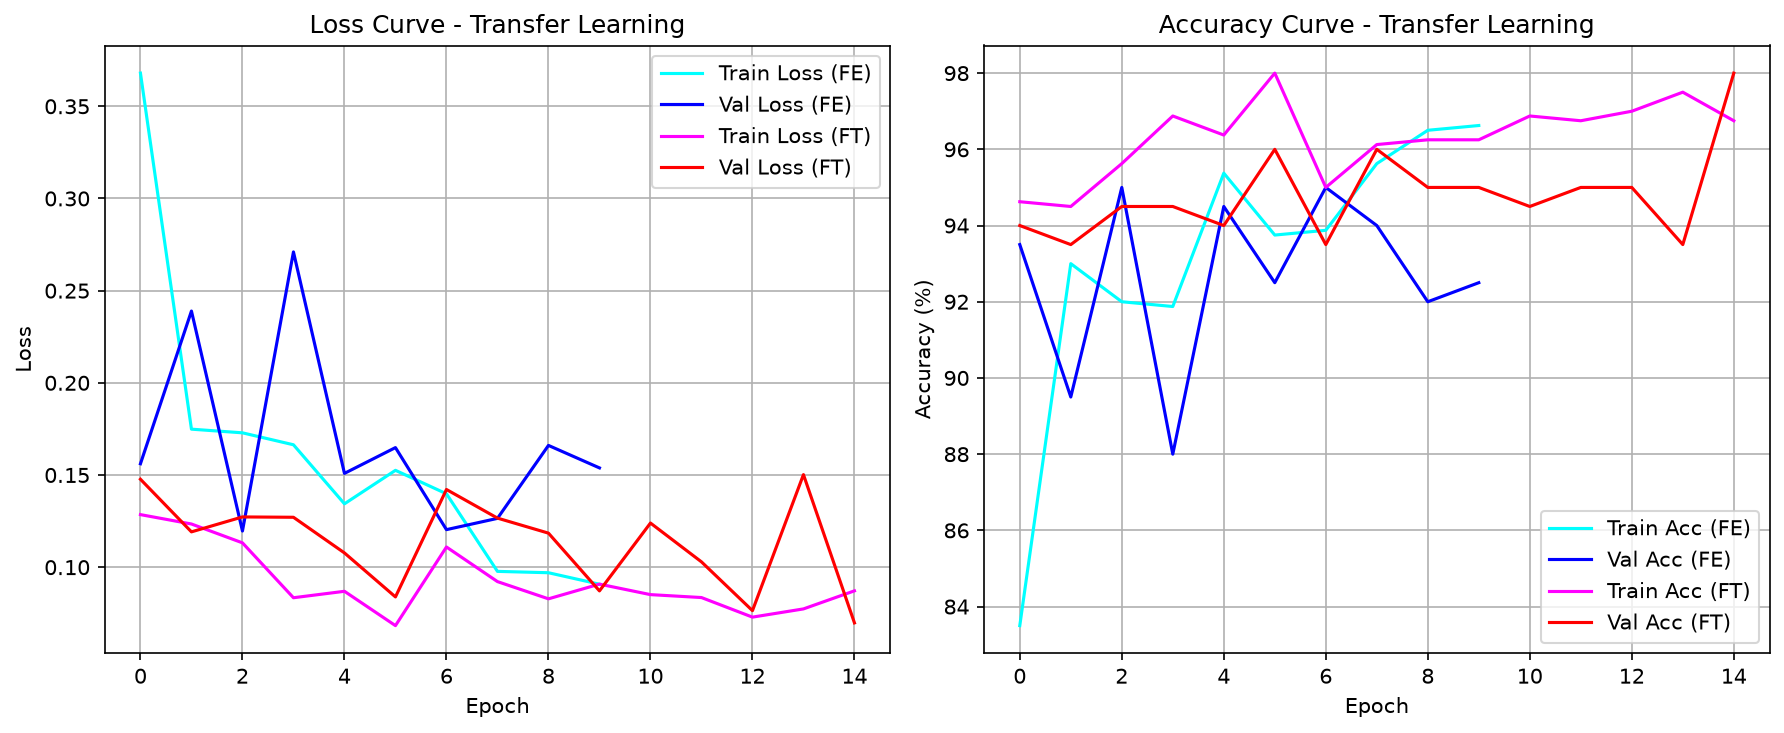
\includegraphics[width=\columnwidth]{figures/transfer_learning_curves.png}
	\caption{Perbandingan loss dan accuracy antara feature extraction (FE) dan fine-tuning (FT).}
	\label{fig:tl_curves}
\end{figure}

\begin{figure}[H]
	\centering
	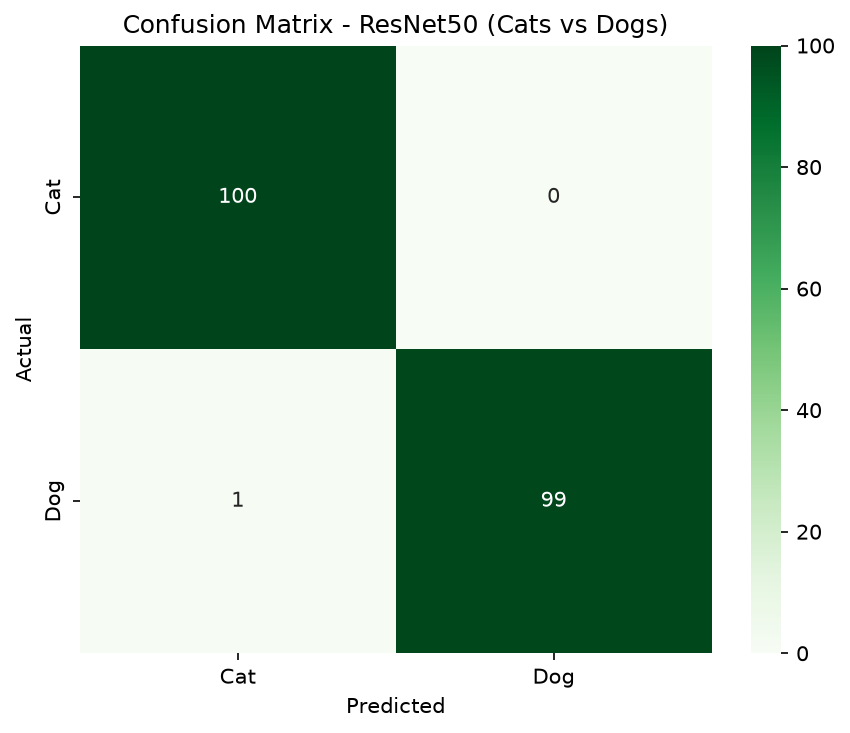
\includegraphics[width=\columnwidth]{figures/confusion_matrix_tl.png}
	\caption{Confusion matrix ResNet50 fine-tuning pada Cats vs Dogs.}
	\label{fig:tl_cm}
\end{figure}

\begin{figure}[H]
	\centering
	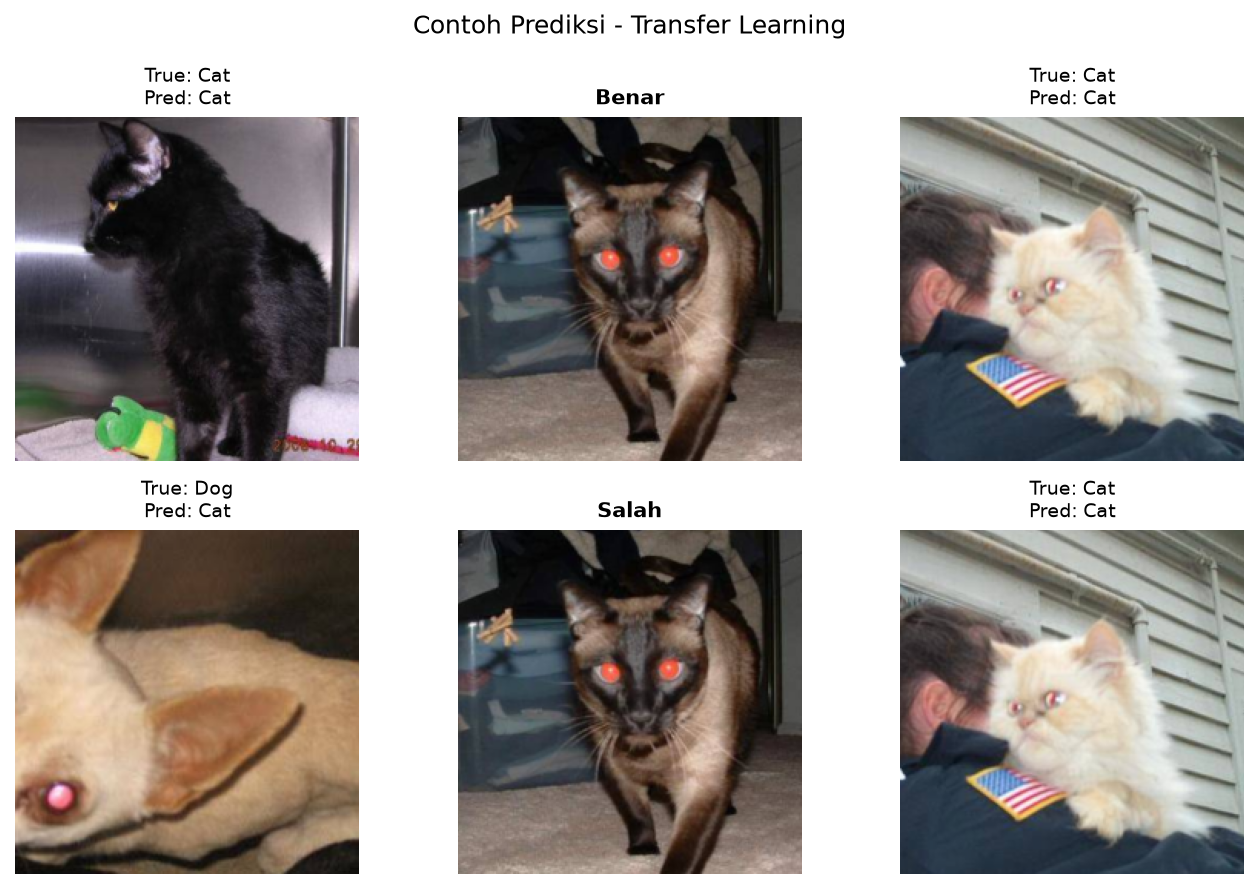
\includegraphics[width=\columnwidth]{figures/predictions_tl.png}
	\caption{Contoh prediksi ResNet50. Model hanya salah memprediksi 1 dari 200 gambar testing.}
	\label{fig:tl_pred}
\end{figure}

Transfer learning menunjukkan performa yang sangat baik:
\begin{itemize}
	\item \textbf{Feature Extraction:} Akurasi testing 99,00\%.
	\item \textbf{Fine-tuning:} Akurasi testing 99,50\%. Hanya 1 dari 200 gambar testing yang salah diklasifikasikan.
\end{itemize}

Fine-tuning memberikan peningkatan 0,5\% dibandingkan feature extraction, menunjukkan bahwa adaptasi bobot pretrained ke dataset target memberikan manfaat tambahan meskipun dataset cukup sederhana.

\section{Perbandingan Model}
Tabel \ref{tab:comparison} menyajikan perbandingan antara CNN from scratch dan transfer learning.

\begin{table}[H]
	\centering
	\caption{Perbandingan CNN from Scratch vs Transfer Learning}
	\label{tab:comparison}
	\resizebox{\columnwidth}{!}{%
		\begin{tabular}{@{}lcc@{}}
			\toprule
			\textbf{Aspek}            & \textbf{CNN from Scratch} & \textbf{Transfer Learning} \\
			\midrule
			Akurasi training          & 76,76\%                   & 96,75\%                    \\
			Akurasi validation        & ~65\% (estimasi)          & 98,00\%                    \\
			Akurasi testing           & 76,76\%                   & 99,50\%                    \\
			Loss training             & 0,741                     & 0,087                      \\
			Loss validation           & 0,732                     & 0,070                      \\
			Waktu training            & ~30 epoch (lebih lambat)  & 10 + 15 = 25 epoch         \\
			Jumlah parameter          & ~535.594                  & ~24.033.090                \\
			Risiko overfitting        & Rendah                    & Rendah--Sedang             \\
			Kemudahan implementasi    & Sedang                    & Mudah                      \\
			Kesesuaian dengan dataset & Cukup (CIFAR-10 umum)     & Sangat baik (2 kelas)      \\
			\bottomrule
		\end{tabular}}
\end{table}

\subsection{Visualisasi Perbandingan}
Gambar \ref{fig:tl_curves} menunjukkan perbandingan kurva loss dan accuracy antara feature extraction dan fine-tuning. Feature extraction menunjukkan konvergensi yang cepat (akurasi validasi > 90\% sejak epoch 1), sementara fine-tuning memberikan peningkatan stabil dari epoch ke epoch.

\section{Analisis}
\subsection{Analisis Dataset}
\textbf{Apakah dataset yang digunakan cukup besar untuk melatih CNN from scratch?}
CIFAR-10 dengan 50.000 gambar training cukup memadai untuk CNN sederhana 2 layer (535K parameter). Rasio parameter terhadap sampel sekitar 10:1, yang berada dalam batas wajar. Namun, untuk arsitektur yang lebih dalam, dataset ini tergolong kecil.

Dataset Cats vs Dogs (1.000 gambar) terlalu kecil untuk melatih CNN from scratch yang baik. Ini dibuktikan dengan dominasi transfer learning yang mencapai 99,5\% akurasi.

\textbf{Apakah variasi gambar sudah cukup baik?}
CIFAR-10 memiliki variasi yang baik dengan 10 kelas berbeda dan 6.000 gambar per kelas. Cats vs Dogs memiliki variasi yang cukup dengan berbagai ras, pose, dan latar belakang.

\textbf{Apakah terdapat ketidakseimbangan data?}
Kedua dataset seimbang. CIFAR-10 memiliki distribusi kelas yang seragam (6.000 per kelas). Cats vs Dogs memiliki jumlah kucing dan anjing yang sama.

\textbf{Apakah gambar memiliki noise, background kompleks, atau variasi pencahayaan?}
CIFAR-10 memiliki resolusi rendah ($32 \times 32$) yang membatasi detail. Cats vs Dogs memiliki resolusi lebih tinggi dengan variasi latar belakang dan pencahayaan yang alami.

\textbf{Bagaimana kualitas dataset memengaruhi hasil?}
Kualitas CIFAR-10 yang stabil dan konsisten membantu CNN from scratch mencapai konvergensi yang baik. Variasi alami Cats vs Dogs diatasi dengan baik oleh representasi pretrained ResNet50 dari ImageNet.

\subsection{Analisis Performa Model}
\textbf{Model mana yang menghasilkan performa terbaik?}
Transfer learning dengan fine-tuning mencapai akurasi testing tertinggi (99,50\%), diikuti feature extraction (99,00\%), dan CNN from scratch (76,76\%).

\textbf{Apakah akurasi tinggi selalu berarti model lebih baik?}
Tidak. Transfer learning diuji pada dataset biner (2 kelas) yang lebih sederhana dibandingkan CIFAR-10 (10 kelas). Akurasi 76,76\% pada 10 kelas setara atau lebih baik dari tebakan acak (10\%). Perbandingan langsung tidak sepenuhnya adil karena perbedaan dataset dan jumlah kelas.

\textbf{Apakah ada tanda-tanda overfitting?}
CNN from scratch menunjukkan loss validasi yang konsisten menurun bersama loss training -- tidak ada indikasi overfitting. Transfer learning dengan 24 juta parameter pada 1.000 gambar berpotensi overfitting, tetapi regularisasi dari pretrained weights dan dropout(0,3) menguranginya secara efektif.

\textbf{Model mana yang lebih stabil selama training?}
Transfer learning lebih stabil dengan fluktuasi minimal. CNN from scratch menunjukkan penurunan loss yang konsisten tetapi lebih lambat.

\subsection{Analisis Pemilihan Pendekatan}
\textbf{Berdasarkan eksperimen, kapan sebaiknya menggunakan CNN from scratch dan kapan sebaiknya menggunakan transfer learning?}

\textbf{Gunakan CNN from scratch ketika:}
\begin{enumerate}
	\item \textbf{Dataset besar} ($>100.000$ gambar): CNN from scratch membutuhkan data yang cukup untuk belajar representasi visual dari nol.
	\item \textbf{Dataset sangat spesifik}: Jika gambar memiliki karakteristik yang sangat berbeda dari ImageNet (misalnya citra satelit, citra medis khusus), pretrained weights mungkin tidak relevan.
	\item \textbf{Kendali penuh atas arsitektur}: Ketika diperlukan arsitektur yang ringan atau khusus untuk deployment di perangkat edge.
	\item \textbf{Tujuan edukasi atau riset}: Untuk memahami mekanisme internal CNN.
\end{enumerate}

\textbf{Gunakan transfer learning ketika:}
\begin{enumerate}
	\item \textbf{Dataset kecil} ($<10.000$ gambar): CNN from scratch akan overfitting. Transfer learning memberikan representasi visual yang sudah matang.
	\item \textbf{Kemiripan dengan ImageNet}: Dataset natural image (objek sehari-hari, hewan, pemandangan) sangat cocok.
	\item \textbf{Keterbatasan komputasi atau waktu}: Transfer learning konvergen lebih cepat (hitungan epoch, bukan ratusan).
	\item \textbf{Target akurasi tinggi}: Pretrained model memberikan akurasi yang sulit dicapai CNN from scratch dengan dataset terbatas.
\end{enumerate}

\section{Studi Kasus Pengambilan Keputusan}
\subsection{Skenario 1: Klinik dengan 300 Gambar Medis}
\textit{CNN from scratch atau transfer learning?}

\textbf{Transfer learning} adalah pilihan yang tepat. Dengan hanya 300 gambar, CNN from scratch hampir pasti overfitting. Pretrained model seperti ResNet50 yang telah belajar dari ImageNet dapat diadaptasi dengan fine-tuning. Untuk citra medis yang sangat berbeda dari ImageNet, disarankan menggunakan model yang telah dipretrain pada dataset medis (seperti CheXNet untuk X-ray) jika tersedia. Feature extraction dengan SVM pada fitur pretrained juga merupakan alternatif yang baik.

\subsection{Skenario 2: Perusahaan dengan 1 Juta Gambar Produk Internal}
\textit{Apakah CNN from scratch masih relevan?}

\textbf{Relevan, tetapi tidak harus eksklusif}. Dengan 1 juta gambar, CNN from scratch dapat dilatih secara efektif. Namun, jika dataset produk memiliki karakteristik yang sangat berbeda dari ImageNet (misalnya gambar industri, mikroskopis), memulai dari scratch bisa menjadi pilihan tepat. Pendekatan optimal: mulai dengan transfer learning (fine-tuning) sebagai baseline, lalu jika performa kurang, lanjutkan dengan CNN from scratch yang diinisialisasi dengan bobot pretrained.

\subsection{Skenario 3: Prototipe 2 Hari dengan 500 Gambar}
\textit{Pendekatan paling rasional?}

\textbf{Transfer learning}. Dalam 2 hari, tidak mungkin melatih CNN from scratch yang baik. Transfer learning memungkinkan:
\begin{itemize}
	\item Loading model pretrained (5 menit)
	\item Feature extraction (1-2 jam training)
	\item Evaluasi dan tuning minimal
\end{itemize}
Dengan 500 gambar, fine-tuning beberapa epoch terakhir saja sudah cukup. Ini adalah pendekatan paling rasional untuk prototyping cepat.

\subsection{Skenario 4: Dataset Besar, GPU Memadai, Domain Spesifik}
\textit{Apakah transfer learning tetap diperlukan?}

\textbf{Tetap diperlukan sebagai initialisasi}. Meskipun dataset besar dan GPU memadai, memulai training dari bobot acak (random initialization) membutuhkan waktu konvergensi yang lebih lama. Transfer learning memberikan:
\begin{itemize}
	\item \textbf{Initialisasi yang lebih baik}: Bobot pretrained sudah berada di area yang baik di loss landscape.
	\item \textbf{Konvergensi lebih cepat}: Fine-tuning dari pretrained weights konvergen lebih cepat dari random initialization.
	\item \textbf{Performa lebih tinggi}: Bahkan dengan dataset besar, initialisasi pretrained sering memberikan hasil akhir yang lebih baik.
\end{itemize}
Pendekatan terbaik: initialisasi dengan pretrained weights, lalu fine-tuning seluruh layer dengan dataset spesifik. Ini menggabungkan kelebihan kedua pendekatan.

\section{Kesimpulan dan Refleksi Pribadi}
Eksperimen ini menunjukkan bahwa transfer learning dengan ResNet50 memberikan performa yang jauh lebih unggul (99,50\%) dibandingkan CNN from scratch (76,76\%) pada dataset yang diuji. Namun, perbandingan ini perlu mempertimbangkan perbedaan kompleksitas dataset (10 kelas vs 2 kelas).

Transfer learning sangat efektif untuk dataset kecil hingga sedang, terutama ketika domain target memiliki kemiripan dengan dataset pretrained. CNN from scratch tetap relevan untuk dataset besar dengan karakteristik unik, serta untuk tujuan edukasi dan riset.

Refleksi pribadi: Eksperimen ini memberikan pemahaman mendalam tentang trade-off antara fleksibilitas arsitektur dan efisiensi pembelajaran. Transfer learning bukanlah solusi universal -- pemilihan pendekatan harus selalu mempertimbangkan konteks spesifik: ukuran dataset, kemiripan domain, ketersediaan komputasi, dan kebutuhan akurasi.

\begin{thebibliography}{1}
	\bibitem{zenodo_catsdogs} T. Boesen, ``dogs\_vs\_cats\_subset\_kaggle,'' Zenodo, Apr. 2024. [Online]. Available: \url{https://zenodo.org/records/10997322}
\end{thebibliography}

\end{document}
